\section{Tikz}
% TODO:https://www.ctan.org/pkg/pgf

\begin{figure}[H]
    \centering
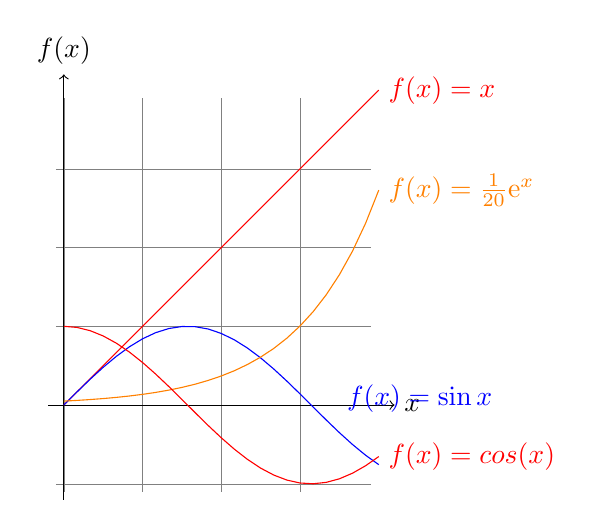
\begin{tikzpicture}[domain=0:4] 
    \draw[very thin,color=gray] (-0.1,-1.1) grid (3.9,3.9);
    \draw[->] (-0.2,0) -- (4.2,0) node[right] {\(x\)};
    \draw[->] (0,-1.2) -- (0,4.2) node[above] {\(f(x)\)};
    \draw[color=red] plot (\x,\x) node[right] {\(f(x)=x\)};
    \draw[color=blue] plot (\x,{sin(\x r)}) node[above=2.4em,right=-1.5em] {\(f(x)=\sin x\)};
    \draw[color=orange] plot (\x,{0.05*exp(\x)}) node[right]
        {\(f(x) = \frac{1}{20} \mathrm e^x\)};
    \draw[color=red] plot (\x,{cos(\x r)}) node[right] {\(f(x)=cos(x)\)};
\end{tikzpicture}
    \caption{some plots}
\end{figure}


Пример с МИСПИСа можно
увидеть на рисунках~\ref{fig:hierarchy_tree}~и~\ref{fig:code_scheme}.

\begin{figure}[H]
    \centering
    \footnotesize
\begin{tikzpicture}[align=center]
\tikzstyle{level 1}=[sibling distance=62mm] 
\tikzstyle{level 2}=[sibling distance=18mm] 
\tikzstyle{level 3}=[sibling distance=16mm] 
\tikzstyle{level 4}=[sibling distance=19mm] 
\node {Ракеты носители РФ}
child { node {ГКНПЦ им.\\М.\:В.\:Хруничева}
    child { node {Ангара} }
    child { node {Протон} 
        child [sibling distance=20mm] { node {Протон-К} 
            child { node {Протон-К --\\Блок ДМ} }
            child [sibling distance=32mm] { node {Протон-К --\\Блок ДМ-2м} }
        }
        child { node{Протон-М} }
    }
}
child { node {ЦСКБ-Прогресс} 
    child { node {Русь} }
    child { node {Р-7} 
        child { node {Спутник} }
        child { node {Луна} }
        child { node {Восток} }
        child { node {Союз}
            child { node {Союз-У} }
            child { node {Союз-ФГ} }
            child { node {Союз-2} }
        }
    }
    child { node {Буря} }
}
child { node {ПО Полет}
    child { node {Космос}
        child { node {Р-12} }
        child { node {Р-14}
            child { node {Космос 3} }
            child { node {Космос-М} }
        }
    }
};
\end{tikzpicture}
\caption{Иерахическое дерево}\label{fig:hierarchy_tree}
\end{figure}

\begin{figure}[H]
    \centering
\begin{tikzpicture}
    \draw (0,4) node [above] {X} -- (0,0) -- (10,0) node [right] {Производитель};
    \draw (2,4) node [above] {X} -- (2,1) -- (10,1) node [right] {Семейство РН};
    \draw (4,4) node [above] {X} -- (4,2) -- (10,2) node [right] {Модель РН};
    \draw (6,4) node [above] {X} -- (6,3) -- (10,3) node [right] {Модификация РН};
\end{tikzpicture}
\caption{Схема структуры кода}\label{fig:code_scheme}
\end{figure}
